\documentclass[../thesis.tex]{subfiles}
  \begin{document}
\chapter{Introduction}\label{cap:introduction}

\section{Background and motivation}
Improving the way an operator can interact with a robot is a hard challenge in the field of \acrfull{HRI}. Nowadays, robots are everywhere, and the control of their movements and actions is usually done through a joystick or a dashboard in the case of very complicated tasks.\\
The idea of using the operator's body to interact with a robot is not a new one, but it brings several challenges when trying to implement it. A possible solution would be to use computer vision and machine learning techniques. In recent years, the computational power of processors and the ability to deploy \acrfull{ML} models on cheaper and smaller devices have paved the way to interact with computers and robots in a way previously unfeasible.

\section{Problem statement}
The main idea of the project is to improve the interaction between humans and robots through computer vision and \acrshort{ML} to detect a set of hand gestures in real time and convey to a robot the action to take in response to the gesture. In this way, the operator can use the expressive power of his/her hands and their immediacy to communicate with the robot. Furthermore, by implementing this concept as an interface using the \acrfull{ROS} framework, we will no longer have to worry about which robot we want to manage in the future; all that is required is that it receives specified messages in order to function. An example of the idea we want to implement is the one in~\ref{fig:systemArchitecture}.

\begin{figure}[H]
  \centering
  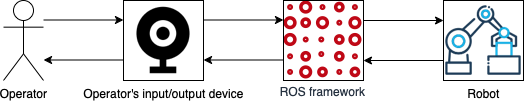
\includegraphics[width=0.7\columnwidth]{thesis/images/systemArchitecture.png}
  \caption{Example of system architecture.}
  \label{fig:systemArchitecture}
\end{figure}

The technology was chosen to be tested in a warehouse scenario because, since 2011, Amazon has been deploying robots within its warehouses, and the number of warehouses using robots to move goods is rapidly increasing~\cite{paper:bogue2016}. In any case, a modular system would make it simple to adjust the robot's activities in response to a gesture or the motions the system recognizes.\\
The system should:
\begin{itemize}
    \item be able to recognize a set of hand gestures;
    \item use the \acrshort{ROS} framework to communicate with a robot;
    \item pick up on new gestures from the user;
    \item create some \glsfirstplural{macro}, save them, and run them;
    \item enables the user to alter the robot's behavior in response to a gesture.
\end{itemize}
To complete all of these tasks, I combed the literature for information on the state of the art of the \acrshort{HRI}, its evaluation methods, and the best way to perform a hand gesture recognition task.

\section{Related works}
In the field of Human-Machine-Interface, there are many attempts to simplify the communication between a human and a machine. Many of them use a third-party device (e.g. a keyboard, a mouse, a controller or a touch screen) to communicate with the machine. This involves a non-immediate understanding of how the controller works, and then the operator must spend some time learning how to use it.\\

A more intuitive way to communicate with a robot is to use some kind of body gesture, mimicking the action that the robot must perform. There are two methods to recognize the gesture and many projects have been built on them~\cite{paper:design_and_evaluate_hand_gesture}:
\begin{itemize}
    \item Vision-based methods: use cameras to capture the reality. The images are analyzed using computer vision and deep learning techniques;
    \item Sensor-based methods: use a third party device like a Wiimote~\cite{paper:guo2008exploring} or a wearable, for example a glove in case of the PowerGlove~\cite{paper:kessler1995evaluation}.
\end{itemize}\\

There are several projects trying to integrate gesture recognition with the control of robots. A particularly interesting one is the one proposed by \citeauthor{paper:chen2019online} in the \citeyear{paper:chen2019online}.  They developed a system composed of three components: an online personal feature pre-training system; a gesture recognition system; and a task re-planning system for robot control~\cite{paper:chen2019online}. Also, searching on GitHub with the keywords ``\textit{robot control gesture}'' returns hundreds of projects, especially related to controlling robotic arms. And, more generally, the task of gesture recognition is a well studied task.\\

It is worth noting that almost all projects are designed to work with a specific robot. The \gls{ROS} is not usually involved, leading to a more difficult integration with future hardware. Moreover, the dynamism of the solution is also not usually taken into account, resulting in a solution that can only be used in that context. In particular, learning a new gesture is usually a difficult task to accomplish.

\section{Organization}\label{s:organization}
This document is organized as follow:
\begin{description}
    \item[{\hyperref[cap:theory]{Chapter two}}] describes the background I obtained studying the literature about \acrlong{HRI}, hand gestures recognition and, \glsfirst{ROS}.
    \item[{\hyperref[cap:methods]{Chapter three}}] describes the technologies and tools used to implement the solution proposed and why they have been chosen to fulfill the requirements. Moreover, the the design process that led to the solution proposed is described. In particular, it is focused on the implementation of the system composed by the hand gesture recognizer and a robot employed in a warehouse (i.e. a storage and retrieval robot).
    \item[{\hyperref[cap:results]{Chapter four}}] presents the results obtained performing several tests with the system developed.
    \item[{\hyperref[cap:discussion]{Chapter five}}] presents a discussion on the results presented in chapter four, explaining them and confronting with other solutions.
    \item[{\hyperref[cap:conclusion]{Chapter six}}] presents my conclusions on the work done for this internship. 
\end{description}

\end{document}
